\section{Configurar el Name Column en una Dimensión}  

1. En las propiedades del atributo Product Key nos ubicamos en NameColumn:

	\begin{center}
	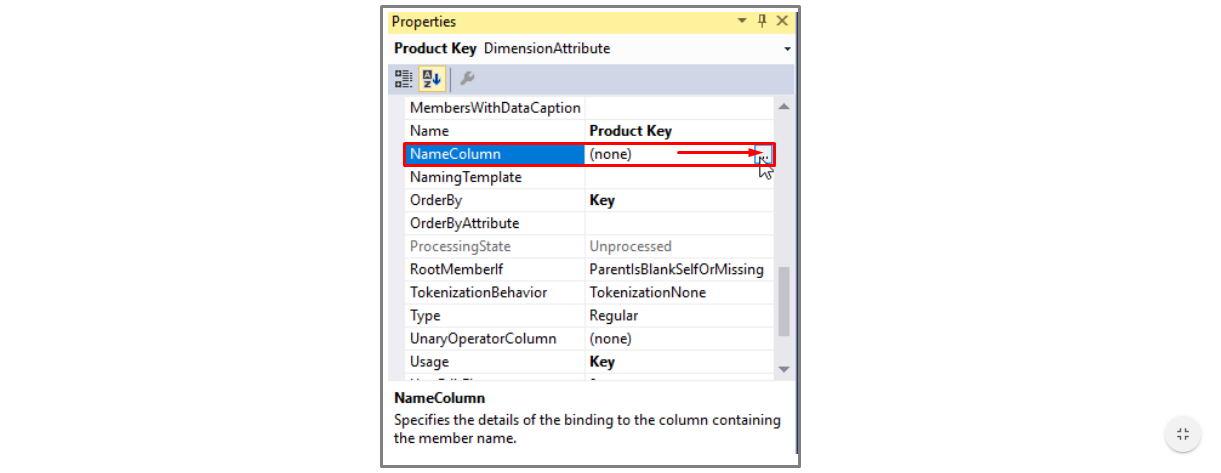
\includegraphics[width=\columnwidth]{images/task1/img1}
	\end{center}	


2. Nos abrirá una ventana donde podemos enmascarar este atributo por otro, en este caso seleccionaremos el
atributo EnglishProductName:

	\begin{center}
	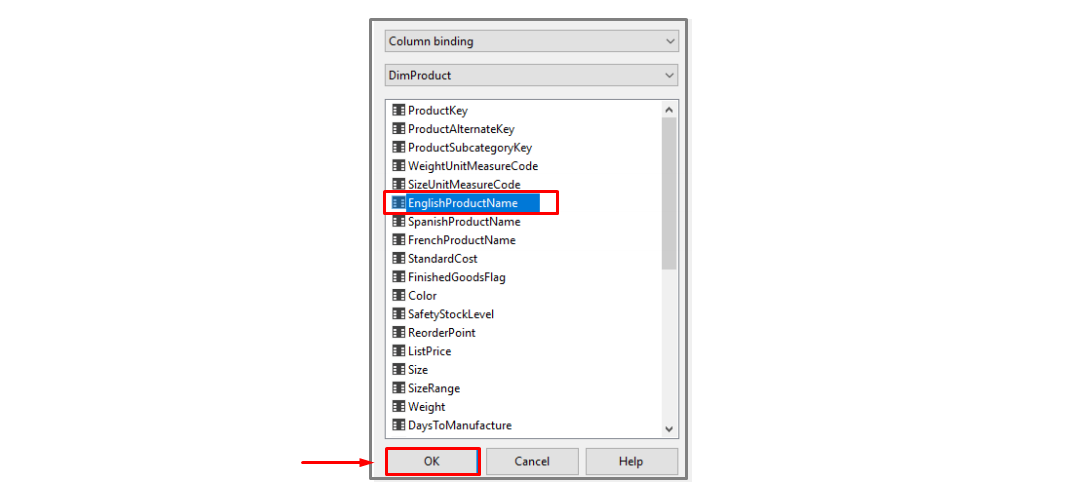
\includegraphics[width=\columnwidth]{images/task1/img2}
	\end{center}	

Click en Ok.

3. Eliminaremos el atributo EnglishProductName y renombraremos el atributo Product Key por Product:

	\begin{center}
	
\includegraphics[width=\columnwidth]{images/task1/img3}
	\end{center}	

Procesamos la dimensión DimProduct.

4. Una vez procesada la dimensión nos volvemos a Reconcetar al mismo:

	\begin{center}
	
\includegraphics[width=\columnwidth]{images/task1/img4}
    \end{center}	

5. Si ahora consultamos el atributo Product obtendremos lo siguiente:

	\begin{center}
	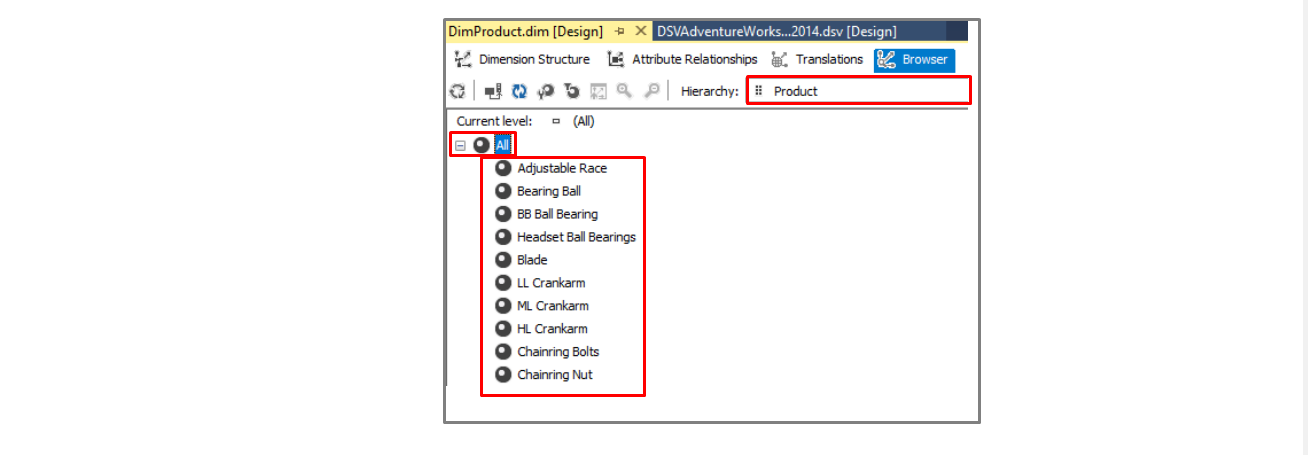
\includegraphics[width=\columnwidth]{images/task1/img5}
    \end{center}	


    